\documentclass[conference]{IEEEtran}
\IEEEoverridecommandlockouts

\usepackage{amsmath}
\usepackage{graphicx}
\usepackage{url}
\usepackage{tikz}
\usepackage{booktabs}
\usetikzlibrary{arrows.meta,positioning,shapes.geometric}

\title{AI-Based Secure CI/CD Pipeline with Risk Scoring}

\author{
\IEEEauthorblockN{Author Name}
\IEEEauthorblockA{Department\\
University\\
City, Country\\
email@domain.com}
}

\begin{document}
\maketitle

\begin{abstract}
We present an AI‑assisted secure CI/CD pipeline implemented in this project and validate it with a full local scan of the same repository. The platform is composed of a React dashboard, a Node.js/Express backend, a Python ML service that performs lightweight scoring, a CI/CD security scanner for workflow and infrastructure artifacts, and a VS Code extension that surfaces findings to developers. A scan executed on April 10, 2026 (UTC) produced an overall CI/CD risk score of 48 (Low) with 45 findings (27 High, 16 Medium, 2 Low), indicating high‑severity issues while remaining below the blocking threshold. The paper documents the implemented architecture, end‑to‑end workflow, and risk‑scoring formulas.
\end{abstract}

\begin{IEEEkeywords}
DevSecOps, CI/CD, risk scoring, vulnerability detection, secure software pipeline, microservices
\end{IEEEkeywords}

\section{Introduction}
CI/CD increases delivery velocity, but it can also accelerate the propagation of insecure configuration, unsafe automation, and vulnerable dependencies. The DevSecOps literature emphasizes continuous security automation across the software lifecycle while noting persistent operational and tooling gaps.\cite{ref_mohammed2025,ref_rajapakse2021,ref_prates2024,ref_zhao2024} ADOC formalizes automated DevSecOps practices in cloud settings.\cite{ref_kumar2020} In this context, the project implements a secure CI/CD pipeline that unifies workflow analysis, infrastructure checks, developer feedback, and backend orchestration. The system spans frontend, backend, ML service, GitHub Actions automation, and a custom CI/CD security scanner. We document the implementation and validate it through a full scan of this repository.

\section{Problem Statement}
There is a need for an end-to-end system that:
1. Automatically scans code, dependencies, CI/CD configuration, and infrastructure files.
2. Produces an interpretable risk score to guide release decisions.
3. Integrates with CI/CD pipelines and developer tooling.
4. Provides dashboard visibility for trends and remediation.

The project targets these goals via a backend orchestration API, a CI/CD security scanner, and a lightweight ML scoring service. Studies of GitHub workflows show limited adoption of security policies and automated checks, which motivates deeper integration of security controls into pipelines.\cite{ref_ayala2023}

\section{Related Work}
Empirical research on CI/CD platforms and GitHub workflows highlights risks around privilege boundaries, token leakage, and action supply‑chain exposure.\cite{ref_koishybayev2022,ref_gu2023,ref_ayala2023} Threat‑modeling work for CI/CD pipelines emphasizes mapping risks to concrete controls and enforcing gates throughout the pipeline.\cite{ref_dhandapani2025} DevSecOps surveys and practice taxonomies consistently identify automated security testing and continuous monitoring as core baseline practices.\cite{ref_mohammed2025,ref_prates2024,ref_zhao2024}

Software supply‑chain security is increasingly guided by frameworks such as NIST SSDF and SLSA, and recent work explores SLSA enablement in workflow systems like Argo.\cite{ref_nist_ssdf,ref_slsa,ref_thariq2025} Practitioner guidance such as the OWASP DevSecOps Guideline adds actionable controls.\cite{ref_owasp_devsecops} AI‑assisted DevSecOps has gained attention, yet surveys stress the need for stronger empirical validation and scalable integration strategies.\cite{ref_binbeshr2025} Studies in SMEs underline practical constraints and the importance of lightweight, automatable controls.\cite{ref_cheenepalli2025}

\section{System Architecture}
The implementation is composed of five components:
1. Frontend dashboard (React, Vite, Tailwind, Recharts) for visualization and management.
2. Backend API (Node.js/Express) for orchestration, authentication, and data services.
3. ML/AI engine (Flask) for rule‑based risk scoring and file analysis endpoints.
4. CI/CD security scanner (\texttt{capci\_cd}) for workflow, IaC, and container checks.
5. Optional data services (MongoDB for persistence; Redis declared in compose but not used in code).

Clients (dashboard, VS Code extension, CI/CD runner) invoke the backend API. The backend runs a repository analyzer (\texttt{main\_analyzer.py}) and the CI/CD scanner, merges findings, stores risks, and exposes reports. Figure~\ref{fig:arch} depicts the deployed components and ports from \texttt{docker-compose.yml}.

\begin{figure*}[htbp]
\centering
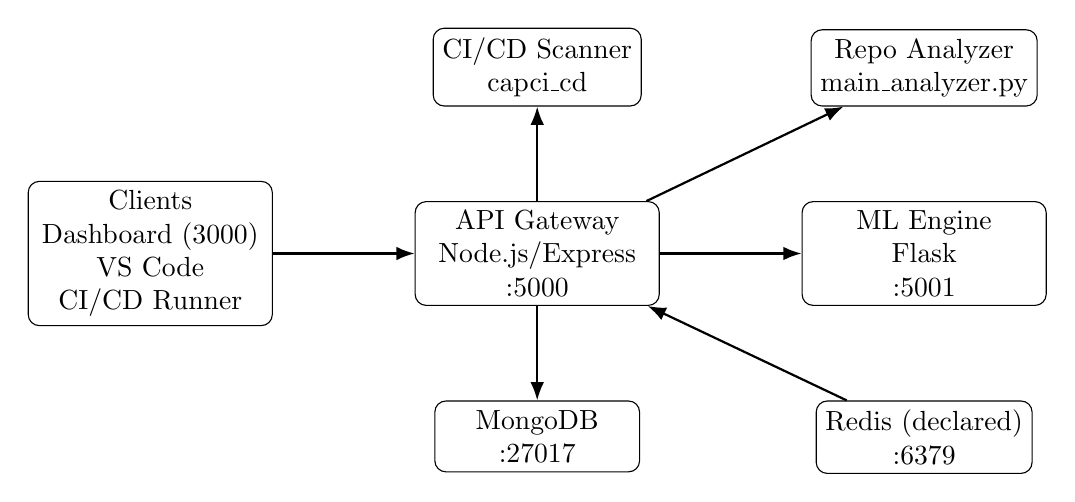
\begin{tikzpicture}[
  node distance=1.2cm and 1.8cm,
  box/.style={draw, rounded corners, align=center, minimum width=3.1cm, minimum height=1.0cm},
  smallbox/.style={draw, rounded corners, align=center, minimum width=2.6cm, minimum height=0.9cm},
  arrow/.style={-Latex, thick}
]
\node[box] (clients) {Clients\\Dashboard (3000)\\VS Code\\CI/CD Runner};
\node[box, right=of clients] (api) {API Gateway\\Node.js/Express\\:5000};
\node[box, right=of api] (ml) {ML Engine\\Flask\\:5001};
\node[smallbox, below=of api] (mongo) {MongoDB\\:27017};
\node[smallbox, below=of ml] (redis) {Redis (declared)\\:6379};
\node[smallbox, above=of api] (scanner) {CI/CD Scanner\\capci\_cd};
\node[smallbox, above=of ml] (analyzer) {Repo Analyzer\\main\_analyzer.py};

\draw[arrow] (clients) -- (api);
\draw[arrow] (api) -- (ml);
\draw[arrow] (api) -- (mongo);
\draw[arrow] (api) -- (scanner);
\draw[arrow] (api) -- (analyzer);
\draw[arrow] (redis) -- (api);
\end{tikzpicture}
\caption{Deployment architecture and ports derived from the project compose file.}
\label{fig:arch}
\end{figure*}

\section{Methodology}

\subsection{Scan Workflow}
The backend scan workflow is implemented in \texttt{backend/src/routes/scans.js}. It launches a Python analyzer, waits for JSON/PDF outputs, then executes the CI/CD scanner against the analyzer’s temporary clone and merges the outputs.

The project also defines a GitHub Actions pipeline that runs the CI/CD scanner and blocks builds if the score exceeds a threshold or if any critical findings are present.

Figure~\ref{fig:flow} summarizes the pipeline flow.

\begin{figure}[htbp]
\centering
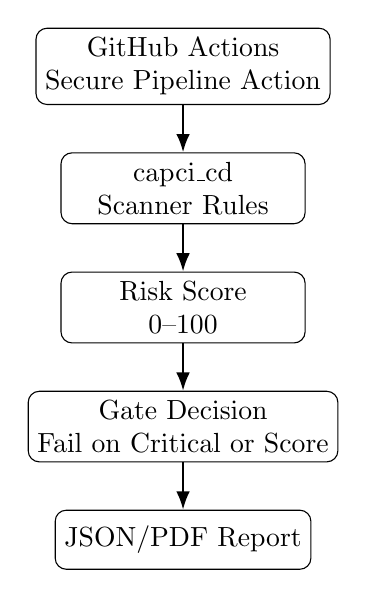
\begin{tikzpicture}[
  node distance=0.6cm,
  block/.style={draw, rounded corners, align=center, minimum width=3.1cm, minimum height=0.75cm},
  arrow/.style={-Latex, thick}
]
\node[block] (gha) {GitHub Actions\\Secure Pipeline Action};
\node[block, below=of gha] (scan) {capci\_cd\\Scanner Rules};
\node[block, below=of scan] (score) {Risk Score\\0--100};
\node[block, below=of score] (gate) {Gate Decision\\Fail on Critical or Score};
\node[block, below=of gate] (report) {JSON/PDF Report};

\draw[arrow] (gha) -- (scan);
\draw[arrow] (scan) -- (score);
\draw[arrow] (score) -- (gate);
\draw[arrow] (gate) -- (report);
\end{tikzpicture}
\caption{CI/CD security scan flow defined in the project action and workflow.}
\label{fig:flow}
\end{figure}

\subsection{Risk Scoring (CI/CD Scanner)}
The CI/CD scanner calculates a weighted score on a 0--100 scale by combining four components: severity, dependency risk, configuration risk, and exposure level. Weights are configured in \texttt{capci\_cd/config.json}.

\begin{equation}
RiskScore_{cicd} = 0.4\cdot S + 0.2\cdot D + 0.2\cdot C + 0.2\cdot E
\end{equation}

Where:
- $S$ is the average severity score (Critical=100, High=75, Medium=45, Low=20).
- $D$ is the dependency/supply-chain risk percentage.
- $C$ is the configuration risk percentage.
- $E$ is the exposure level percentage.

The CI/CD pipeline blocks builds when the overall risk score is $\geq 80$ or when any critical issue is detected.

\subsection{Risk Scoring (ML Service)}
The ML service uses a rule‑based function that normalizes weighted findings to a 0--10 score and maps that score to a risk level.

\begin{equation}
RiskScore_{ml} = \min\left(10, \frac{\sum_i w_i\cdot c_i}{10}\right)
\end{equation}

The service exposes \texttt{/api/analyze}, \texttt{/api/score}, and \texttt{/api/dependencies} for code and dependency checks.

\section{Implementation}

\subsection{Frontend Dashboard}
The dashboard is built with React (Vite + Tailwind), uses Recharts for visualization, and relies on Zustand for state management. It integrates with backend endpoints that provide projects, scans, risks, and pipeline metrics.

\subsection{Backend API}
The backend exposes REST endpoints for authentication, projects, scans, risks, pipelines, and dashboard metrics. It supports JWT-based auth and OAuth providers via Express sessions, and persists data in MongoDB when configured.

\subsection{CI/CD Security Scanner}
The scanner analyzes GitHub Actions workflows, Dockerfiles, Compose files, Kubernetes manifests, and Terraform/IaC. It flags risks such as overly permissive permissions, unpinned actions, privileged containers, exposed secrets, and public cloud resources. Findings are exported as JSON and PDF reports.

\subsection{Developer Tooling}
The VS Code extension provides commands for workspace or file scans, submits requests to configured API endpoints, and renders inline diagnostics.

\section{Results and Discussion}
We executed a full CI/CD scan of the repository locally on April 10, 2026 (UTC) using \texttt{capci\_cd/run\_secure\_pipeline.py}. The scan produced a risk score of 48 (Low) with 45 total issues (27 High, 16 Medium, 2 Low) across 17 files. The most frequent categories were Privilege Escalation (19), Unauthorized Access (10), and Data Exposure (9).

Table~\ref{tab:eval} summarizes the measured results and runtime in this environment.

\begin{table}[htbp]
\centering
\caption{Repository Scan Summary (April 10, 2026 UTC)}
\label{tab:eval}
\begin{tabular}{lcc}
\toprule
\textbf{Metric} & \textbf{Value} & \textbf{Source} \\
\midrule
Overall risk score & 48 (Low) & capci\_cd report \\
Total issues & 45 & capci\_cd report \\
High / Medium / Low & 27 / 16 / 2 & capci\_cd report \\
Scan runtime & 9.93 s & local run \\
External tool findings & 0 recorded & capci\_cd report \\
\bottomrule
\end{tabular}
\end{table}

The CI/CD scan includes files under \texttt{capci\_cd}, \texttt{capci\_cd\_extracted}, and \texttt{temp\_repo} that contain example IaC and container configurations intentionally crafted to trigger policy checks. This increases the issue count and should be separated from production repositories in future evaluations.

\section{Limitations}
1. The ML service relies on rule-based heuristics rather than a trained model.
2. External tools (e.g., \texttt{pip-audit}, \texttt{semgrep}, \texttt{trivy}) run only if installed; no external findings were recorded in this scan.
3. The repository analyzer expects a Git URL and clones into \texttt{temp\_repo}; it does not natively scan an on-disk path.
4. Redis is declared in compose but is not integrated into backend logic and therefore remains unused.

\section{Future Work}
1. Integrate a trained ML model for calibrated risk classification.
2. Add persistent queueing for scan orchestration (Redis/Bull or similar).
3. Separate example IaC artifacts from production scans to reduce noise.
4. Add automated performance benchmarks for scan duration and API latency.

\section{Conclusion}
This paper described the secure CI/CD pipeline implementation, its scan workflow, and the measured results from a full repository scan. The system combines a backend orchestrator, a CI/CD security scanner, a rule‑based ML scoring service, and developer tooling. It enforces pipeline gates using a 0--100 risk score and emits consolidated JSON/PDF reports, providing a practical baseline for future data‑driven improvements.

\section*{Acknowledgment}
The authors thank the project team for implementation and testing support.

\begin{thebibliography}{00}
\bibitem{ref_koishybayev2022} I. Koishybayev, A. Nahapetyan, R. Zachariah, S. Muralee, B. Reaves, A. Kapravelos, and A. Machiry, ``Characterizing the Security of Github CI Workflows,'' in \emph{Proc. 31st USENIX Security Symposium}, 2022. \url{https://www.usenix.org/system/files/sec22-koishybayev.pdf}
\bibitem{ref_gu2023} Y. Gu, L. Ying, H. Chai, C. Qiao, H. Duan, and X. Gao, ``Continuous Intrusion: Characterizing the Security of Continuous Integration Services,'' in \emph{Proc. IEEE Symp. on Security and Privacy}, 2023. \url{https://xgao-work.github.io/paper/sp2023_2.pdf}
\bibitem{ref_kumar2020} R. Kumar and R. Goyal, ``Modeling continuous security: A conceptual model for automated DevSecOps using open-source software over cloud (ADOC),'' \emph{Computers \& Security}, vol. 97, 101967, 2020. doi:10.1016/j.cose.2020.101967.
\bibitem{ref_prates2024} L. Prates and R. Pereira, ``DevSecOps practices and tools,'' \emph{International Journal of Information Security}, 2024. doi:10.1007/s10207-024-00914-z.
\bibitem{ref_mohammed2025} K. I. Mohammed, B. Shanmugam, and J. El-Den, ``Evolution of DevSecOps and Its Influence on Application Security: A Systematic Literature Review,'' \emph{Technologies}, vol. 13, no. 12, 548, 2025. doi:10.3390/technologies13120548.
\bibitem{ref_rajapakse2021} R. N. Rajapakse, M. Zahedi, M. A. Babar, and H. Shen, ``Challenges and solutions when adopting DevSecOps: A systematic review,'' \emph{arXiv preprint} arXiv:2103.08266, 2021. \url{https://arxiv.org/abs/2103.08266}
\bibitem{ref_ayala2023} J. Ayala and J. Garcia, ``An Empirical Study on Workflows and Security Policies in Popular GitHub Repositories,'' \emph{arXiv preprint} arXiv:2305.16120, 2023. \url{https://arxiv.org/abs/2305.16120}
\bibitem{ref_dhandapani2025} S. Dhandapani, ``Enhancing Software Supply Chain Security Through STRIDE-Based Threat Modelling of CI/CD Pipelines,'' \emph{arXiv preprint} arXiv:2506.06478, 2025. \url{https://arxiv.org/abs/2506.06478}
\bibitem{ref_thariq2025} M. Thariq and I. Ekanayake, ``ARGO-SLSA: Software Supply Chain Security in Argo Workflows,'' \emph{arXiv preprint} arXiv:2503.20079, 2025. \url{https://arxiv.org/abs/2503.20079}
\bibitem{ref_binbeshr2025} F. Binbeshr and M. Imam, ``Comparative Analysis of AI-Driven Security Approaches in DevSecOps: Challenges, Solutions, and Future Directions,'' \emph{arXiv preprint} arXiv:2504.19154, 2025. \url{https://arxiv.org/abs/2504.19154}
\bibitem{ref_cheenepalli2025} J. Cheenepalli, J. D. Hastings, K. M. Ahmed, and C. Fenner, ``Advancing DevSecOps in SMEs: Challenges and Best Practices for Secure CI/CD Pipelines,'' \emph{arXiv preprint} arXiv:2503.22612, 2025. \url{https://arxiv.org/abs/2503.22612}
\bibitem{ref_zhao2024} X. Zhao, T. Clear, and R. Lal, ``Identifying the primary dimensions of DevSecOps: A multi-vocal literature review,'' \emph{Journal of Systems and Software}, vol. 214, 112063, 2024. doi:10.1016/j.jss.2024.112063.
\bibitem{ref_nist_ssdf} NIST, ``Secure Software Development Framework (SSDF) Version 1.1,'' NIST SP 800-218, 2022. \url{https://csrc.nist.gov/pubs/sp/800/218/final}
\bibitem{ref_slsa} OpenSSF, ``Supply-chain Levels for Software Artifacts (SLSA),'' 2023. \url{https://slsa.dev/spec/v1.0/whats-new}
\bibitem{ref_owasp_devsecops} OWASP, ``DevSecOps Guideline,'' 2024. \url{https://owasp.org/www-project-devsecops-guideline/}
\end{thebibliography}

\end{document}
